\section{GitHub}
\label{sec.github}


\begin{figure}[h]
  \centering
  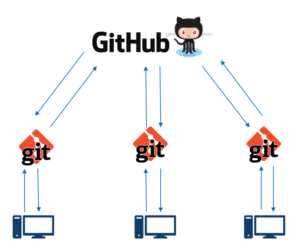
\includegraphics[width=0.5\textwidth]{GitHub-How-to-use-GitHub-Edureka-300x241.png}
%%  \url{https://www.edureka.co/blog/how-to-use-github/}
  \caption{GitHub is a cloud service that hosts code repositories which 
    you can access via a web browser.}
\end{figure}

\subsection{Objectives}
The assignment in this section is:
\begin{enumerate}
\item Create a GitHub account
\item Open the \code{src/hello.py} with GitHub Codespaces.
\item Run the \emph{tests}  in \code{tests/test\_hello.py}using Codespaces
\end{enumerate}

\subsection{Overview}

For this atelier you will use \textbf{GitHub CodeSpaces} as your
development environment.  This is a cloud-based interactive
development environment (IDE).  If you are interested in continuing to
work on the project after the atelier is finished today, you will
still be able to access GitHub CodeSpaces for as long as you wish in
the coming days, months, years.



You will start with existing code in a central repository of code, hosted by
GitHub on the cloud.  You will download (clone) a copy of this
repository, edit existing code, and create new code.

GitHub is a web based service which hosts thousands of projects, small
and large, in the cloud.  Typically, users have a development
environment on their local computer (laptop or desktop) and
periodically upload and download changes to the cloud.

The URL \url{https://github.com/jimka2001/immersion}, is the public
entry point to the GitHub project which we will work on in this
atelier.

You must create an account on GitHub (if you don't have one already).
This will be done in Section~\ref{sec.setup}.


\subsection{Getting Started}
\label{sec.setup}

We recommend you use the Chrome web browser.


\includegraphics[width=0.5\textwidth]{chrome.png}.

We need to set up the development environment.  The following steps should
help.

\subsection{Account Creation}
  
Create a GitHub account using an abstract user name.  Don't use your
real name.  Instead use an artificial name use as your name from
instagram or other social media.  You may also make up a completely
new name as long as no other person has already used that name on
GitHub.  \url{https://github.com/join}.  To complete the process of
creating a GitHub account you may need to authenticate using your
mobile phone.


\noindent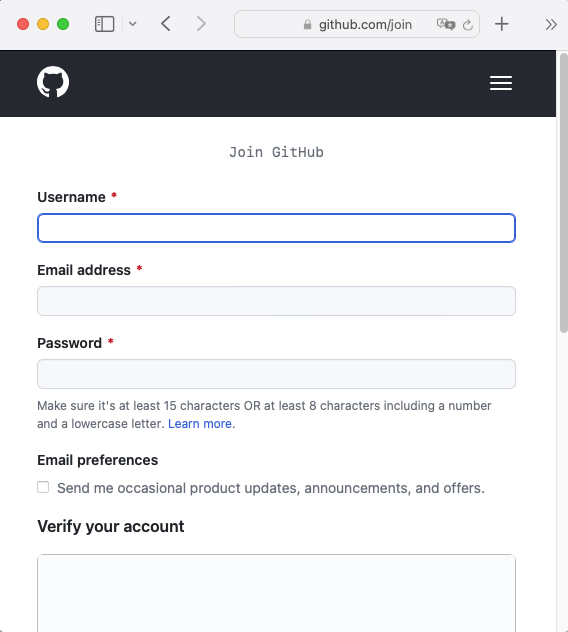
\includegraphics[width=0.5\textwidth]{github-join.png}



\subsection{Open the Repository}
  
Open \url{https://github.com/jimka2001/immersion} with your web browser.

\noindent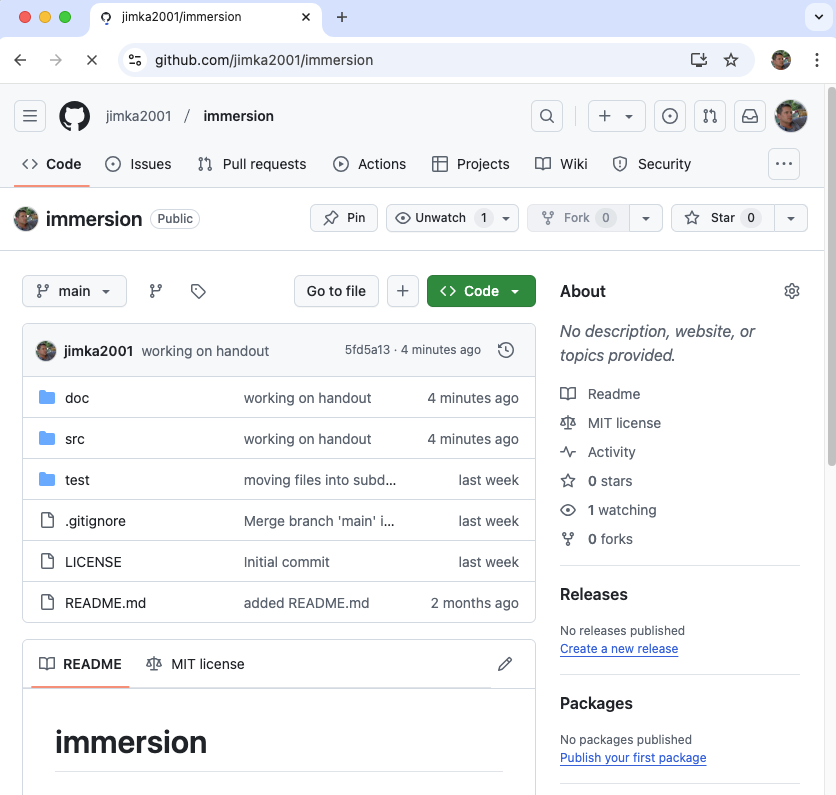
\includegraphics[width=0.5\textwidth]{github-immersion.png}


\subsection{Fork yourself a copy}

Fork the repository.  This gives you a private copy.  You will make changes
necessary changes in the code using this private copy.

\noindent 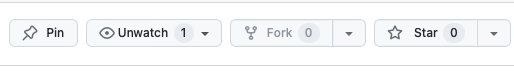
\includegraphics[width=0.6\textwidth]{github-fork-repo.png}



\subsection{Open a Python File in Codespaces}
  
\begin{enumerate}
\item Navigate to \code{src/hello.py} to see something like this.

\noindent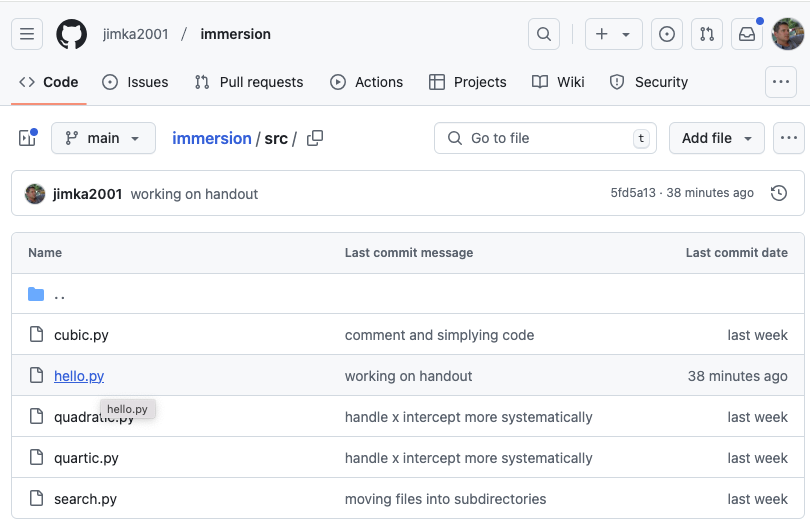
\includegraphics[width=0.9\textwidth]{find-hello.png}



\item Click \code{hello.py} to open the file in an editor pane.  You
  should see something like what is shown here:

\noindent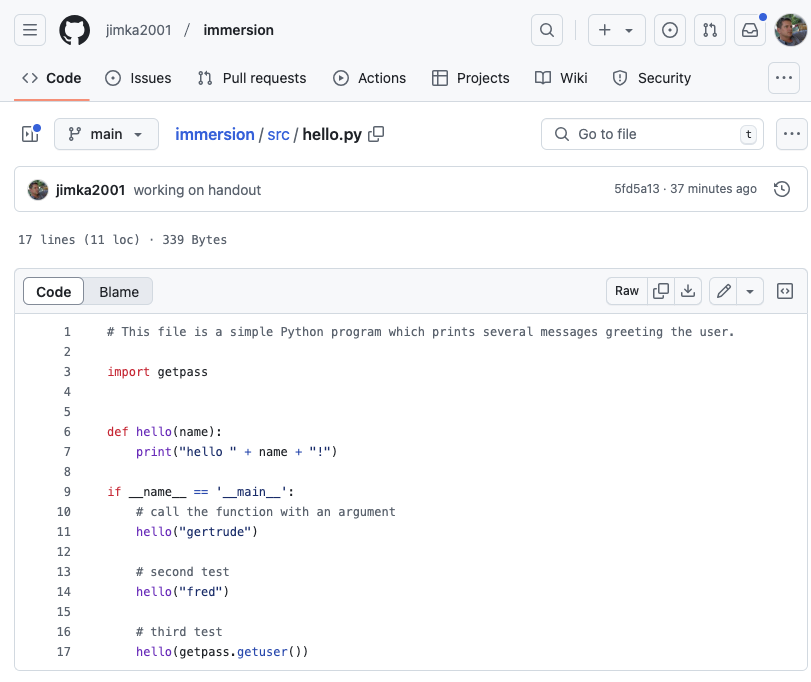
\includegraphics[width=0.9\textwidth]{hello-function.png}


\item Open the file by clicking \code{github.dev} not \code{Edit in place}.

\noindent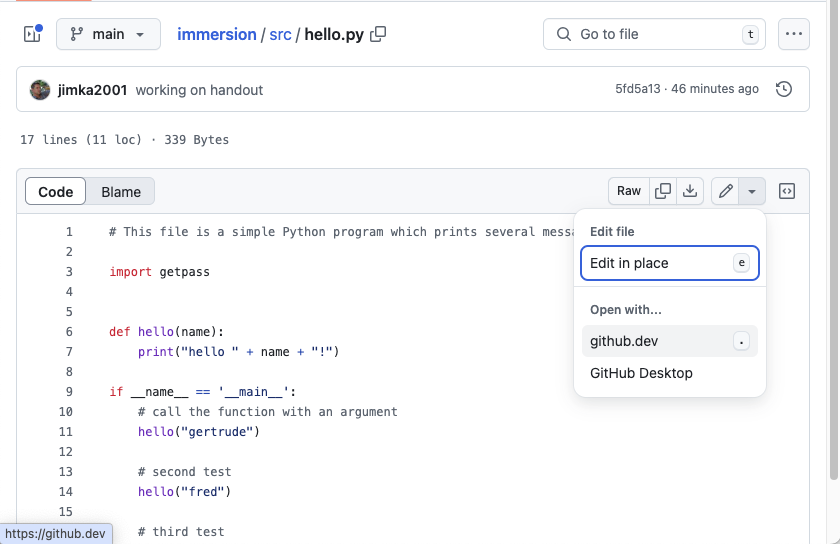
\includegraphics[width=0.9\textwidth]{github-dev.png}


\item You may need to wait while setting up. If this setup seems to
  never finish, it may mean you need to use Chrome as your web
  browser.

\noindent
\includegraphics[width=0.4\textwidth]{github-dev-setup.png}


\item GitHub may ask for permission to see your repository.  Click on \textbf{Allow}.
  
\noindent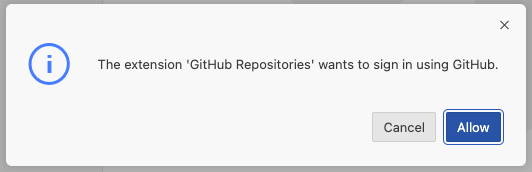
\includegraphics[width=0.7\textwidth]{github-ask-permission.png}
  

\item GitHub may ask for your GitHub ID.  Normally you just select the default one.
  
\noindent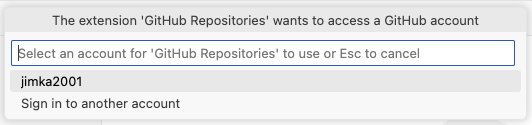
\includegraphics[width=0.5\textwidth]{github-ask-user-name.png}

\item Finally, the GitHub development environment should be opened.
  
\noindent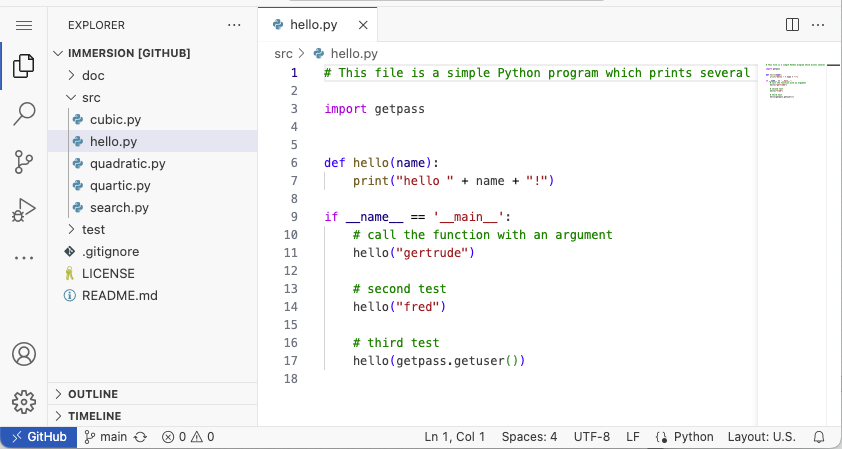
\includegraphics[width=0.6\textwidth]{github-dev-opened.png}



\end{enumerate}

\subsection{Set up the Editor}
  
\begin{enumerate}

\item Now you can edit your code but you cannot run nor test it.

\item Find the icon 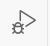
\includegraphics[width=2cm]{run-debug.png} on the left hand side of the browser window.   Press that icon to see the following message.

\noindent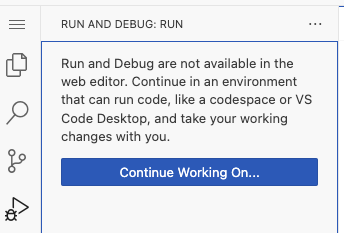
\includegraphics[width=0.6\textwidth]{continue.png}

\item Press continue, and you should see a prompt such as the following to create a code space.   

\noindent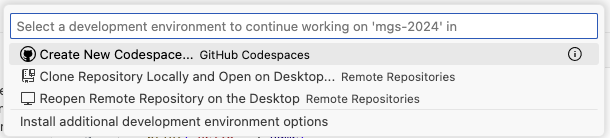
\includegraphics[width=0.9\textwidth]{create-code-space.png}

\item Select 
\includegraphics[width=8cm]{select-create.png}.

\item You may be asked how many cores do you want.

\noindent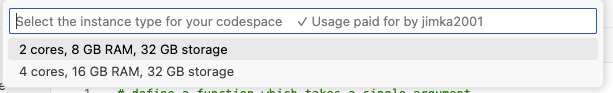
\includegraphics[width=0.9\textwidth]{select-cores.png}

\item You should select the minimum: 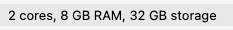
\includegraphics[width=7cm]{two-cores.png}.

\item You'll probably now need to reopen the \code{src/hello.py} file.

\noindent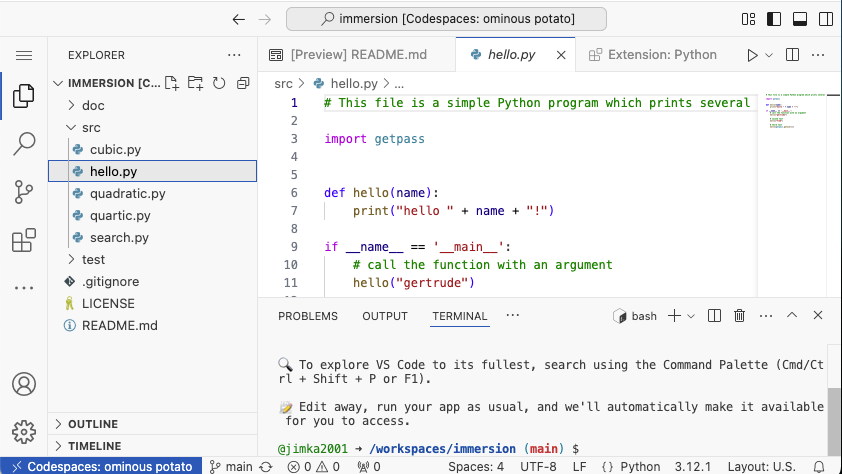
\includegraphics[width=0.9\textwidth]{re-open-python-file.png}

\item You may be asked to install the Python extension.  Press \textbf{Install}.

\noindent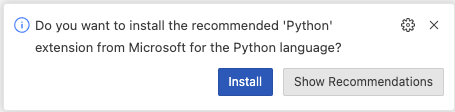
\includegraphics[width=0.8\textwidth]{install-python-extension.png}

  

\item Wait until it finishes installing.  When it finishes installing, you should see something like this:

\noindent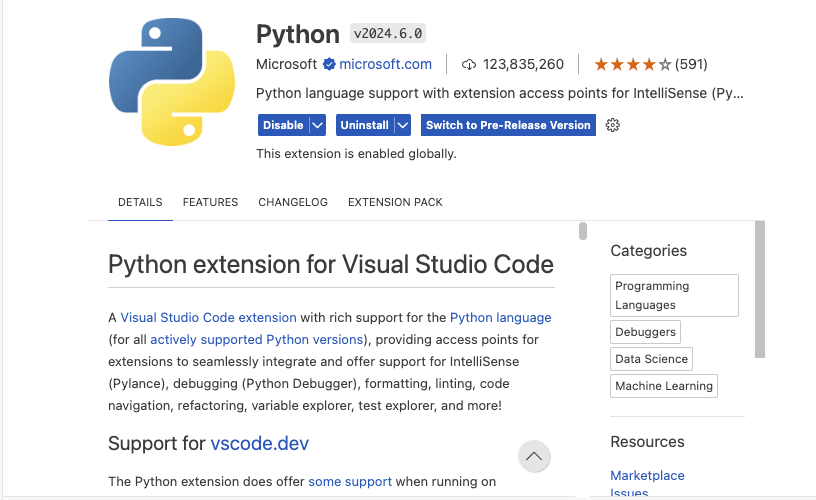
\includegraphics[width=0.9\textwidth]{python-extension.png}

\item Reopen the explorer: 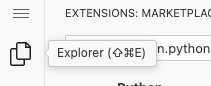
\includegraphics[width=7cm]{explorer2.png}, and select the \code{src/hello.py} file.

\noindent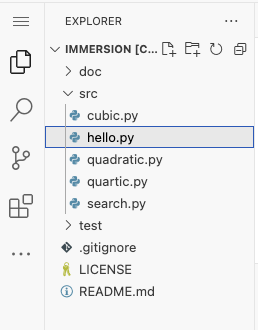
\includegraphics[width=0.4\textwidth]{explorer.png}
\end{enumerate}

\subsection{Example the Code}
Take a look at the Python code in the file \code{src/hello.py}.  In particular there are two sections in the code, 
\begin{enumerate}
\item A declaration of the function named \code{hello}, shown in Listing~\ref{list.hello}
\item Two conditional calls to the function \code{hello}, each time with a different argument, shown in Listing~\ref{list.calls}.
\end{enumerate}

\begin{listing}{Declaration of Function \code{hello}}{hello}
\begin{minipage}[c]{0.95\textwidth}\begin{lstlisting}
def hello(name):
    print("hello " + name + "!")
\end{lstlisting}\end{minipage}\end{listing}

\begin{listing}{Calls to Function \code{hello}}{calls}
\begin{minipage}[c]{0.95\textwidth}\begin{lstlisting}
if __name__ == '__main__':
    # call the function with an argument
    hello("gertrude")
    
    # second test
    hello("fred")
\end{lstlisting}\end{minipage}\end{listing}


\subsection{Make a Sample Run}

Find the icon 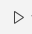
\includegraphics[height=1.0cm]{run-triangle.png}
  in the top-right of the editor window.  Click the triangle, to see a sample run/execution of the code.

\noindent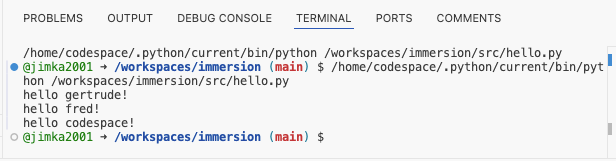
\includegraphics[width=\textwidth]{hello-terminal-output.png}


\subsection{Running Predefined Tests}
\label{sec.run.tests}

Open the file \code{tests/test\_hello.py} in a GitHub Codespace.

\noindent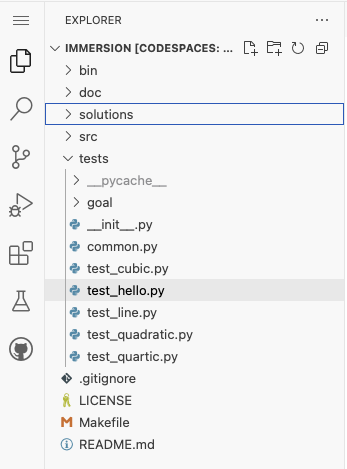
\includegraphics[width=0.4\textwidth]{test-hello-explorer.png}

To run the tests, press the 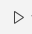
\includegraphics[width=1cm]{run-triangle.png} which
you should find in the upper-right corner of the editor window.

\noindent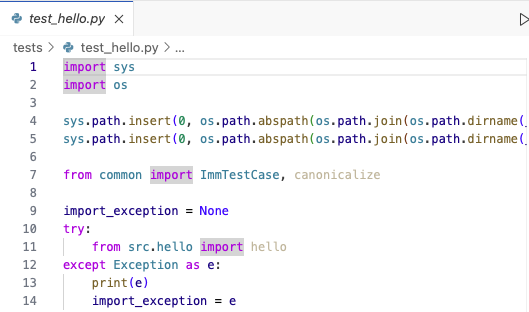
\includegraphics[width=0.8\textwidth]{hello-test.png}


The text window at the bottom of the editor should show the results of
how many tests ran and whether there are any failures.

\noindent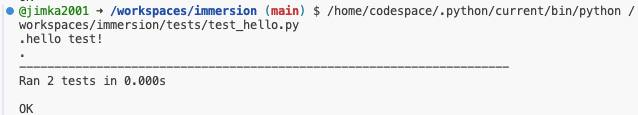
\includegraphics[width=0.8\textwidth]{github-test-result.png}



\subsection{Challenges for the Student}

Understanding errors and debugging is difficult, but it is part of programming.

Experiment with the simple pieces of code in the above sections.
Insert spaces and press the run button.  Look at the error messages
produced. Remove some quotation marks or parentheses (leaving
unbalanced quotations marks or parentheses)---again look at what error
messages you see when you try to run invalid code.


\begin{enumerate}
\item Remove and add some spaces at the beginning of a line.
\item Change the indentation.
\item Unbalance the parentheses.
\item Unbalance the quotation marks.
\item Put extra spaces inside the quotation marks.
\item Change the name of the \code{hello} function at definition site or call site.
\item Figure out how to undo your changes in the editor to make the code work again.
\item Run the tests \code{test/test\_hello.py} as explained in Section~\ref{sec.run.tests}.
\end{enumerate}

\clearpage

